\section{Patrones de Diseño Adapter} 
\textbf{}\\
\begin{flushleft}
El patrón de diseño Adapter es utilizado cuando tenemos interfaces de software incompatibles, las cuales a pesar de su incompatibilidad tiene una funcionalidad similar. Este patrón es implementado cuando se desea homogeneizar la forma de trabajar con estas interfaces incompatibles, para lo cual se crea una clase intermedia que funciona como un adaptador. Esta clase adaptador proporcionará los métodos para interactuar con la interface incompatible.


	\begin{center}
	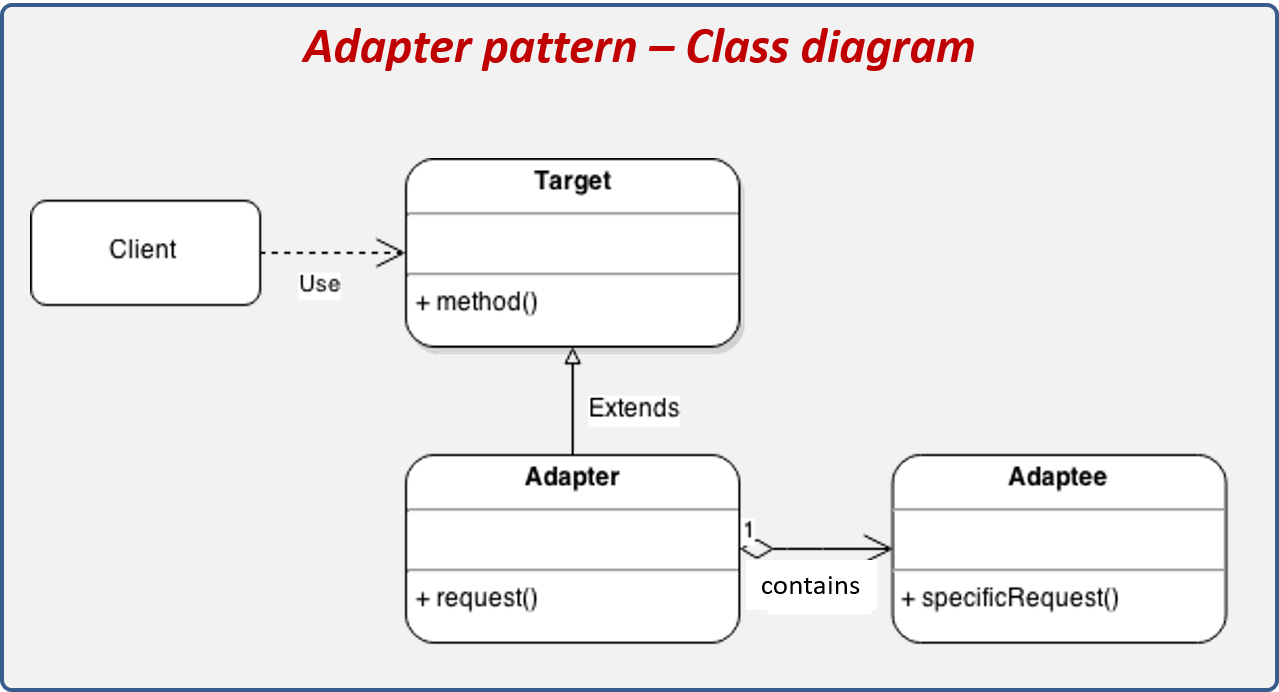
\includegraphics[width=10cm]{./Imagenes/adapter} 
	\end{center}

\textbf{  Los componentes que conforman el patrón son los siguientes:}\\
\begin{enumerate}[a)]
\item Client: Actor que interactua con el Adapter.
\item Target: Interface que nos permitirá homogenizar la forma de trabajar con las interfaces incompatibles, esta interface es utilizada para crear los Adapter.
\item Adapter: Representa la implementación del Target, el cual tiene la responsabilidad de mediar entre el Client y el Adaptee. Oculta la forma de comunicarse con el Adaptee.
\item Adaptee: Representa la clase con interface incompatible.
                                                                                                                                                                                                             
\newpage


\end{enumerate}
         \begin{center}
	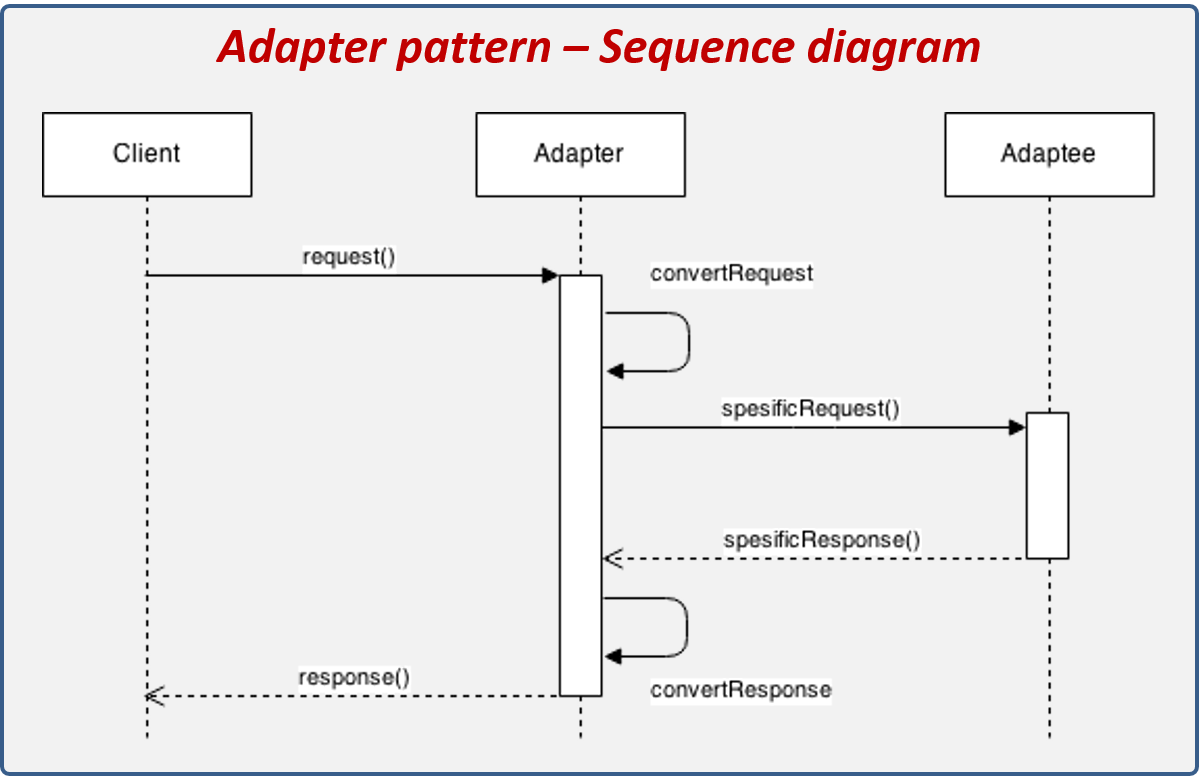
\includegraphics[width=10cm]{./Imagenes/adapter2} 
	\end{center}
\vfill

\begin{enumerate}[a)]
\item El Client invoca al Adapter con parámetros genéricos.
\item El Adapter convierte los parámetros genéricos en parámetros específicos del Adaptee.
\item El Adapter invoca al Adaptee.
\item El Adaptee responde.
\item El Adapter convierte la respuesta del Adaptee a una respuesta genérica para el Client.
\item El Adapter responde al Client con una respuesta genérica.
\end{enumerate}
\vfill
\textbf{         EJEMPLO DEL MUNDO REAL}
\\ Mediante la implementación del patrón de diseño Adapter crearemos un adaptador que nos permite interactuar de forma homogénea entre dos API bancarías, las cuales nos permite aprobar créditos personales, sin embargo, las dos API proporcionadas por los bancos cuenta con interfaces diferentes y aunque su funcionamiento es prácticamente igual, las interfaces expuestas son diferentes, lo que implica tener dos implementaciones diferentes para procesar los préstamos con cada banco. Mediante este patrón crearemos un adaptador que permitirá ocultar la complejidad de cada implementación del API, exponiendo una única interface compatible con las dos API proporcionadas, además que dejáramos el camino preparado por si el día de mañana llegara una nueva API bancaría.
          \begin{center}
	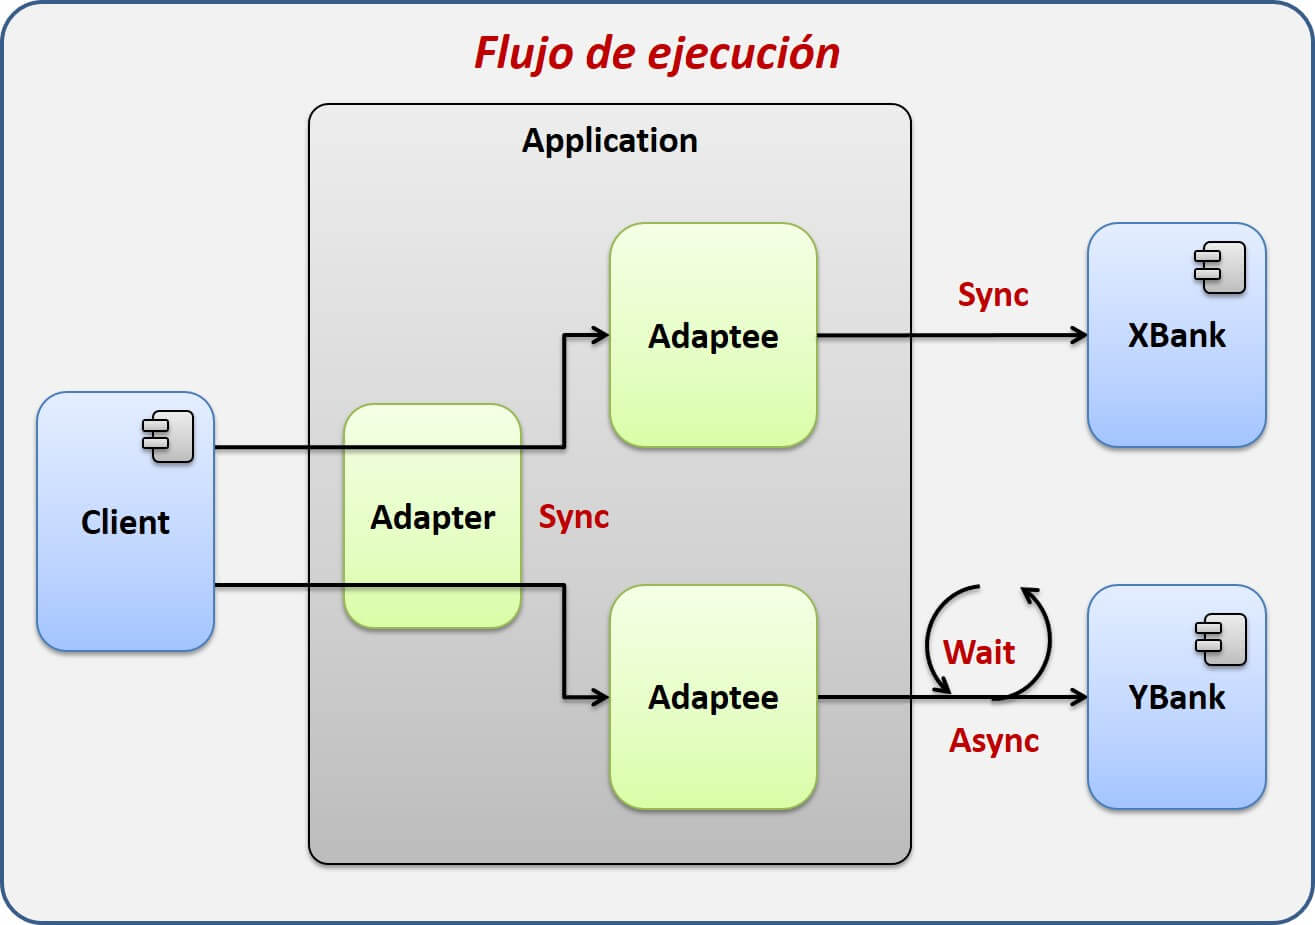
\includegraphics[width=10cm]{./Imagenes/adapter3} 
	\end{center}
	




\end{flushleft}
